\documentclass[utf8,xcolor=table]{beamer}

\usepackage[T2A]{fontenc}
\usepackage[utf8]{inputenc}
\usepackage[english,russian]{babel}
%\usepackage{tikz-uml}
\usepackage{minted}
\usepackage{cmap}

\hypersetup{colorlinks,linkcolor=blue,urlcolor=blue}

\mode<presentation>{
	\usetheme{CambridgeUS}
}

\renewcommand{\t}[1]{\ifmmode{\mathtt{#1}}\else{\texttt{#1}}\fi}
\newcommand{\svgimg}[1]{
  \begin{center}
	\includegraphics[scale=1]{#1.pdf}
  \end{center}
}

\title[Git]{Системы контроля версий и Git}
\author{Егор Суворов}
\institute[НИУ ВШЭ]{Курс <<Основы программирования>>}
\date[14.11.2019]{Четверг, 14 ноября 2019 года}

\setlength{\arrayrulewidth}{1pt}

\begin{document}

\begin{frame}
\titlepage
\end{frame}

% !TeX root = 191114.tex
\section{Зачем СКВ?}
\begin{frame}[t]{Воспроизводимость}
\textbf{Код и требования часто меняются}
\begin{itemize}
\item Код будет разрабатываться и запускаться на разных компьютерах
%	\begin{itemize}
%	\item Даже если пишете проект только для себя: переустановка/смена ОС, потеряли компьютер, обновились...
%	\end{itemize}
\item Требуется, чтобы код можно было разрабатывать и запускать где угодно
%	\begin{itemize}
%	\item В идеале: скачали нечто, нажали одну кнопку, есть готовый проект в IDE для разработки
%	\item Обычно ограничиваются подробным README и использованием стандартных инструментов для сборки
%	\item Надо явно прописать что запускать, как собирать, какие нужные файлы в каких местах, какие библиотеки нужны...
%	\end{itemize}
\item Можно автоматизировать проверку и тестирование на разных компьютерах!
%\item Иначе можно скачать код и обнаружить:
%	\begin{itemize}
%	\item Нехватку файлов для компиляции
%	\item Запускается только в одной конкретной папке
%	\item Работает только если Python находится в конкретной папке
%	\item Работает только если открыть в PyCharm и настроить папочки определённым образом
%	\end{itemize}
\item Чтобы достичь воспроизводимости, требуется вкладывать время и соблюдать процессы
	\begin{itemize}
	\item Это может казаться "избыточным" на одном компьютере
	\item Если внезапно потребуется, добавлять воспроизводимость больнее, чем делать с начала
	\end{itemize}
%\item Пример: https://github.com/yeputons/csc-gpgpu-fall-2018-tasks
\end{itemize}
\end{frame}

\begin{frame}[t]{Контроль версий "--- разработка}
\textbf{Код и требования часто меняются}

Иногда хочется самому:
\begin{itemize}
\item Вернуть всё на последнюю рабочую версию
\item Посмотреть, что поменялось
\item Понять, откуда взялась странная строчка
\item Сделать много изменений, а потом перепроверить их по отдельности
\item Попробовать сделать сложное изменение (Микадо-метод)
%  \item Возможно, несколькими способами
%  \item И чтобы можно было быстро между ними переключаться
\end{itemize}

При работе в команде:
\begin{itemize}
\item Все пункты выше особенно важны, потому что нет общего контекста
\item Несколько людей меняют один файл
\item Кто-то меняет несколько файлов согласованно (\verb~.h~ и \verb~.cpp~), надо обновлять пачкой
\item Понять логику изменений за время отпуска
\end{itemize}
\end{frame}

\begin{frame}[t]{Контроль версий "--- развёртывание}
При развёртывании ПО:
\begin{itemize}
\item Точно знать, какой код сейчас запущен на сервере
\item Точно знать, какой код был запущен на сервере позавчера
\item Указывать версии нужных библиотек
\item Автоматически следить за номерами версий
\end{itemize}

Иначе можно:
\begin{itemize}
\item Не понять, где произошла ошибка: логи указывают на место, которого в текущем коде нет
\item Взять у коллеги только один обновлённый файл, остальные остаются старыми => не компилируется
\item Не понять, почему весь код поменялся за неделю и начать активно расспрашивать коллег
\item Не вспомнить, откуда взялась строчка, и бояться её убрать (вдруг важная)
\end{itemize}
\end{frame}

\begin{frame}[t]{Контроль версий "--- процессы}
Чтобы контролировать версии, требуется вкладывать время и соблюдать процессы
\begin{itemize}
  \item Это тоже может казаться "избыточным", если вы работаете один
  \item Но лучше вырабатывать привычку, в неожиданный момент пригождается
  \item Если внезапно потребуется, добавить контроль версий невозможно. Только с конкретного момента времени.
\end{itemize}
\end{frame}

\begin{frame}[t,fragile]{Система контроля версий}
Система, которая позволяет вам все хотелки (в идеале) и:
\begin{itemize}
\item Хранит все версии вашего кода
\item Позволяет между ними переключаться
\item Позволяет смотреть на изменений
\item Даёт удалённый доступ к коду (например, для команд)
\end{itemize}
Примеры: Git, Mercurial, SVN...

<<Общая папка>> (email, dropbox, флешки, сетевой диск) сюда не попадает:
надо руками создавать версии (\verb~main4.cpp~), копировать всю папку, это муторно. 
\end{frame}

\begin{frame}[t]{Версии и коммиты}
\begin{itemize}
\item Система хранит несколько независимых \textit{репозиториев} ($\approx$ папка с историей)
\item История "--- набор отдельных версий (\textit{коммитов})
\item Ещё \textit{коммитом} называют изменение между версией и предыдущей
\item На коммиты делит программист.
\item Каждый коммит "--- атомарное по смыслу изменение, в идеале:
	\begin{itemize}
	\item Есть хорошее короткое описание коммита
	\item Можно целиком откатить изменения, ничего не сломав
	\item Можно взять любую версию и код в адекватном состоянии
	\end{itemize}
\item Почему не автоматически делить на коммиты?
\end{itemize}
\end{frame}

\begin{frame}[t]{Как делить на коммиты}
Отдельно:
\begin{itemize}
\item Автоматические (одна команда в IDE: переименовать метод)
\item Механические: обернуть все вызовы во что-то.
%    * Make Callback's SharedString a const ref.
%      https://github.com/apache/incubator-pagespeed-mod/commit/338c37915355c0a4dd8726643cd90718bc394d6f#diff-f227b6faa8dc001f2312dadc7d72e53c
\item Содержательное: новая функциональность, исправление бага.
\end{itemize}
Постоянно следите за репозиторием:
\begin{itemize}
\item Про каждое изменение рассказать, зачем оно было сделано
%  * Чтобы потом можно было не спрашивать коллег (которые уволились), а читать историю
%  * https://habr.com/ru/post/416887/
\item Должно быть можно откатываться между версиями
%  * Никогда заранее не знаешь, куда захочешь откатиться, поэтому лучше делить на маленькие коммиты
%  * Но не слишком маленькие, чтобы можно было осмысленно откатиться плюс-минус к любому коммиту
%    * Деление "изменил имя функции в a.txt/b.txt" - плохое, потому что нельзя откатиться в середину
\end{itemize}

%* Сделали несколько изменений одновременно - несколько разных коммитов
%  * А вдруг в каком-то баг? Тогда можно будет проще найти, в каком
%  * Склеивать коммиты проще, чем разделять
%* За репозиторием надо постоянно следить! "Поправить потом" очень больно и скорее невозможно
%* Если что-то неудобно - спросите, наверняка можно настроить и добавить в привычку
%  * Нельзя делать отладочный вывод, который не отключён по умолчанию
%  * Нельзя читать из файлов по захадкоженному пути
\end{frame}

\begin{frame}[t]{Ветки}
Часто надо вести несколько \textit{веток} разработки:
\begin{itemize}
\item
	Несколько человек добавляют разные независимые фичи и что-то постоянно ломают.
\item 
	Хочется провести эксперимент и не ломать основную версию кода.
\end{itemize}
\end{frame}

% !TeX root = 191114.tex
\begin{frame}[t]{Книжка про Git}
Pro Git, второе издание:
\begin{center}
\href{https://git-scm.com/book/ru/v2/}{git-scm.com/book/ru/v2}
\end{center}
\end{frame}

\begin{frame}[t]{Git vs SVN}
\begin{itemize}
\item SVN "--- типичная \textit{централизованная} система: один сервер, на котором хранится вся история (SVN), локально только текущая.
	\begin{itemize}
	\item История может быть большой.
	\item Для работы нужно подключение к серверу.
	\item Можно сделать сквозную нумерацию коммитов
	\end{itemize}
\item Git "--- типичная \textit{децентрализованная} система: на каждом отдельном компьютере хранится вся история.
	\begin{itemize}
	\item Синхронизация через специальный условно-центральный компьютер.
	\item История должна помещаться на компьютер.
	\item Можно работать без сервера вообще.
	\item Генерировать номера коммитов сложно.
	\end{itemize}
\end{itemize}
	Другие особенности:
\begin{itemize}
\item В Git всё \textit{очень} хорошо с \textit{ветками}, их удобно и просто делать
\item Git сейчас модный: хостинги, инструменты, интеграции...
\item Следствие: Git проще начать пользоваться
\end{itemize}
\end{frame}

\begin{frame}[t]{Распределённые системы контроля версий}
\begin{center}
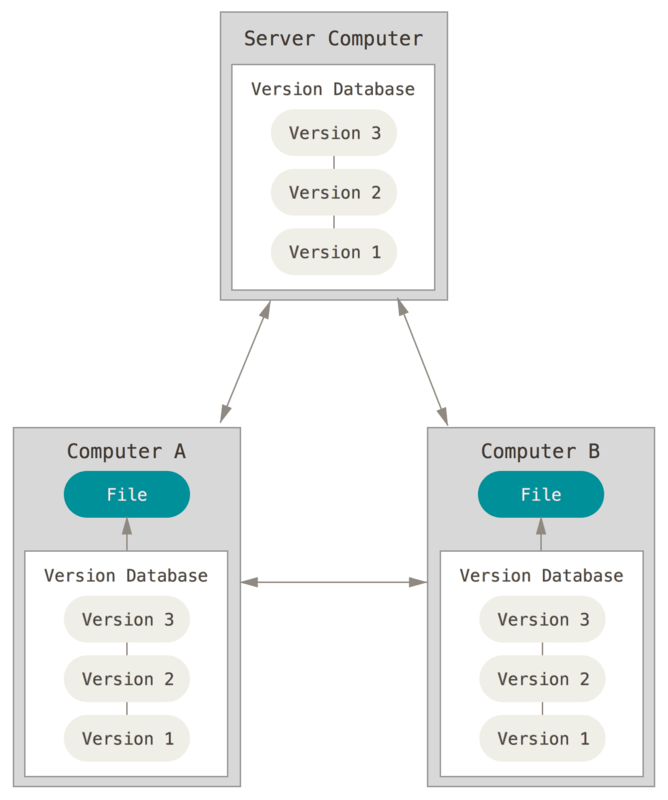
\includegraphics[height=0.8\textheight,keepaspectratio]{distributed.png}
\end{center}
\end{frame}

\begin{frame}[t]{Git vs GitHub}
Git:
\begin{itemize}
\item Система контроля версий.
\item Консольный клиент.
\end{itemize}
GitHub:
\begin{itemize}
\item Хостинг для git-репозиториев.
\item Добавляет \textit{pull requests}.
\item Добавляет \textit{интерфейс} для code review.
\item Даёт <<из коробки>> интеграции с другими инструментами.
\end{itemize}
Можно пользоваться Git без GitHub, это нормально.
\end{frame}

\begin{frame}[t]{Модель данных Git}
\begin{itemize}
\item Каждый \textit{commit} "--- отдельная версия.
\item У коммита есть \textit{предыдущий} (или несколько) "--- \textit{parent}.
\item Получаем ацикличный граф (демо ungit!)
\item \textit{Branch} (ветка) "--- указатель на комммит, двигается.
\item \textit{Tag} (тэг) "--- указатель на коммит, не двигается.
\item \textit{Remote} "--- другой репозиторий, с которым
	можно синхронизироваться (на другом компьютере).
\end{itemize}
Тонкости:
\begin{itemize}
\item Отслеживаются только файлы, не папки.
\item Отслеживается только содержимое файлов (переименование..?).
\item Никак не проверить автора или время коммита.
\item Имя коммита "--- хэш от содержимого.
\item Синхронизация "--- просто скачали себе данные в \verb~remote/ветка~,
	ветки и история локально не меняются.
\end{itemize}
\end{frame}

\begin{frame}[t]{Состояние репозитория в Git}
\begin{center}
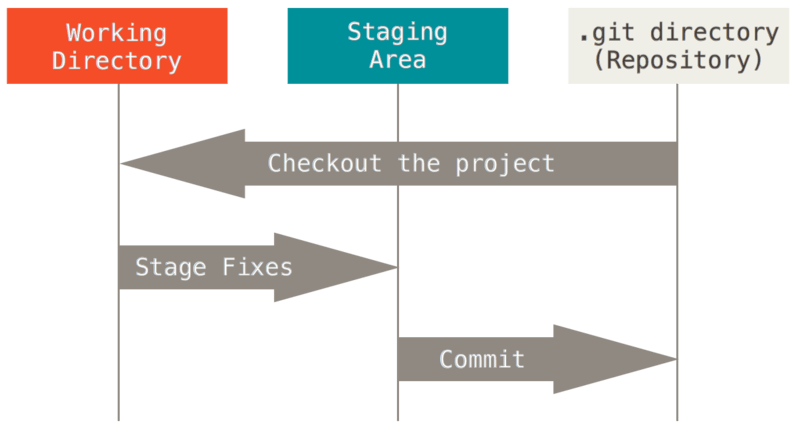
\includegraphics[width=\textwidth,keepaspectratio]{areas.png}
\end{center}
\end{frame}

\begin{frame}{Состояния файлов}
\verb~git status~
\begin{center}
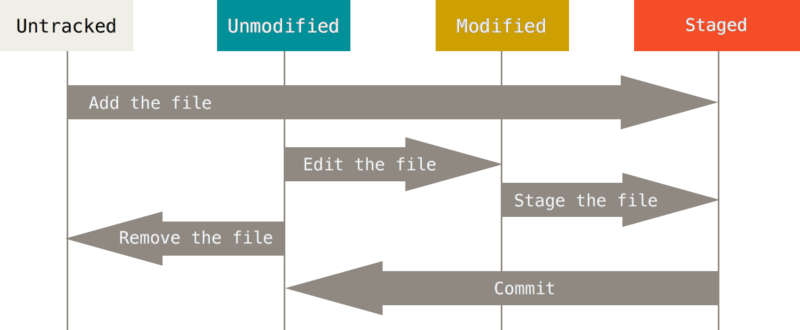
\includegraphics[width=\textwidth,keepaspectratio]{lifecycle.png}
\end{center}
\begin{itemize}
\item Ещё есть \textit{игнорирование}, оно влияет, если файл \textit{untracked}.
\item Файл может быть и \textit{modified}, и \textit{staged}.
\end{itemize}
\end{frame}

\begin{frame}{Слияние веток}
\begin{center}
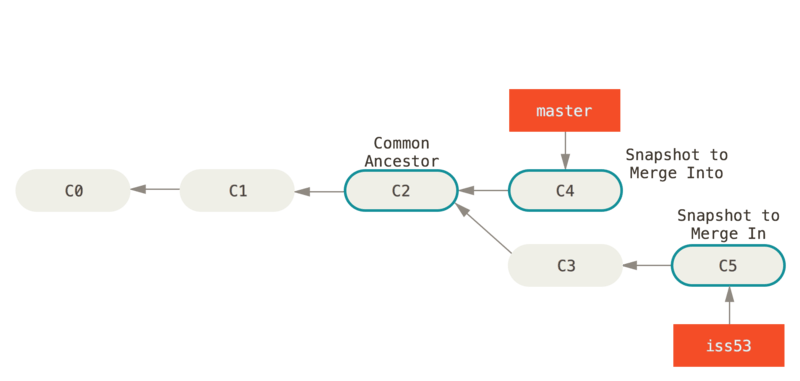
\includegraphics[width=\textwidth,keepaspectratio]{basic-merging-1.png}
\end{center}
\end{frame}


\end{document}
